%%% Endowing the Pisa/IIT SoftHand with the sense of touch

\subsubsection{Endowing the Pisa/IIT SoftHand with the sense of touch}
\label{sec:SenseOfTouch}


\noindent $\blacktriangleright$  \textbf{Hardware} \\ 
\newline

In this section the sensors will be described and how these was managed and used in the application . The information about acceleration, angular rotation velocity and  magnetic field can be obtained by an IMU (Inertial Measurements Unit).  The low power, light weight and potential for low cost manufacture of these units opens up a wide range of solution. The  purpose is to constrain rigidly one device on each phalanges of the fingers, more two  on the palm of the hand.  Although the size of a generic IMU is very small, the selection  was accurate to permit the correct assembly on the hand. Thus an Invensence product has been chosen, MPU-9250.  \\
\newline

\noindent $\bullet$ \textbf{MPU-9250}

\noindent The MPU-9250 is a System in Package (SiP) that combines two chip: the MPU-6500 (used for the paper published in ICRA2015), wich contains a 3-axis gyroscope, a 3-axis accelerometer, and an onboard Digital Motion Processor (DMP); and AK8963, the market leading 3-axis digital compass.  
\begin{figure}[h]
\centering
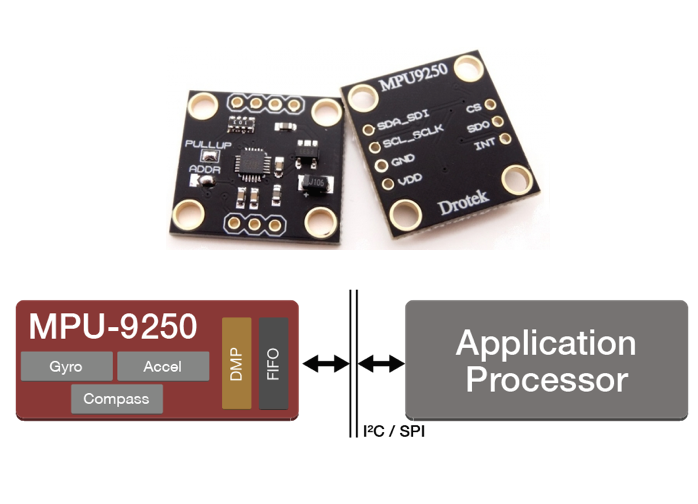
\includegraphics[scale=0.35]{mpu9250.png}
\caption{MPU-9250}
\label{fig:mpu9250}
\end{figure}

\begin{itemize}
\item[$\cdot$] \textit{Accelerometer}: the MPU-9250's accelerometers use separate proof masses for each axis. Acceleration along a particular axis induces displacement on the corresponding proof mass, and capacitive sensors detect the displacement differentially. The 3-analog informations are digitized using individual on-chip 16-bit Analog-to-Digital Converers(ADCs) to sample each axis;

 \item[$\cdot$] \textit{Gyroscope}: three indipendet vibratory rate gyroscopes are in the MPU-9250, wich detect rotation about the X, Y and Z axes. When the gyroscope are rotated about any of sense axes, the Coriolis Effect causes a ibration that is detected by a capacitive pickoff. The resulting signal is amplified, demodulated and filtered to produce a voltage that is proportional to the angular rate. This voltage pass thorugh a ADC providing digital outputs.

 \item[$\cdot$] \textit{Magnetometer}: the 3-axis magnetometer uses higly sensitive Hall sensor technology. It detects terrestrial magnetism in the X, Y and Z axes. As the other, each ADC has 16-bit resolution. 
\end{itemize}


\noindent The MPU-9250's technical features are summarized in the table \ref{tab:mpu}.
\begin{table}[tb]\footnotesize
\caption{MPU-9250 features}
\centering
\label{tab:mpu}
\begin{tabular}{l | c | l}
\textbf{Part} & \textbf{Unit} &  \\ \hline \hline
Gyro Full Scale Range & (deg/sec) &  $\begin{array}{l}   \pm 250 \\  \pm 500  \\ \pm 1000 \\ \pm \textbf{2000} \end{array}$  \\   
\rowcolor [gray]{.8}  \text{Gyro Rate Noise} &  (\text{dps}/$\sqrt{\text{Hz}}$)  & $\begin{array}{l}   0.01 \end{array}$  \\ 
\text{Accel Full Scale Range} & (\text{g}) & $\begin{array}{l}   \pm 2 \\  \pm 4 \\  \pm \textbf{8} \\ \pm 16 \end{array}$ \\ 
\rowcolor [gray]{.8} \text{Compass Full Scale Range} &($\mu\text{T}$) & $\begin{array}{l}   \pm \textbf{4800} \end{array} $\\ 
\text{Digital Output} &  & $\begin{array}{l} \text{I}^2\text{C} \\ \textbf{SPI}   \end{array} $ \\  
\rowcolor [gray]{.8} \text{Logic Supply Voltage } & (\text{V}) & $\begin{array}{l} 1.7\text{V}\text{to}\text{VDD} \\ \textbf{VDD}   \end{array} $\\ 
\text{Package Size} & (\text{mm}) & $\begin{array}{l} 3\text{x}3\text{x}1   \end{array}$ 
\end{tabular}
\end{table}


The output data from  axes sensors can be read,  in digital way, from a 8-bit  register of the device.  Each axis sensor presents two registers,   up  and  low register. Thus a complete information from a specific sensor, e.g. the accelerometer, occupies 32-bit. 

The figure \ref{fig:axes} shows the orientation of the axes of sensitivity and the polarity of rotation.
\begin{figure}[h]
\centering
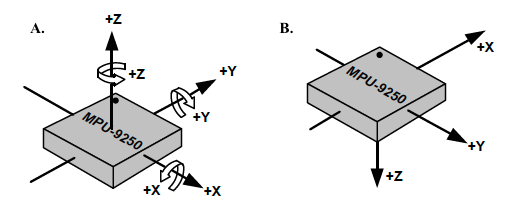
\includegraphics[scale=0.5]{axes_orientation.png}
\caption{A. accelerometer and gyro orientation axes  B. magnetometer oreintation axes}
\label{fig:axes}
\end{figure}

The necessary IMU to compute the complete posture of the hand are 17, 15 applied on each phalanges and 2 on the palm of the  hand. 
In this way the communication and data sending to a processing unit becomes a  crucial aspect. In the MPU-9250 it is possible to select two different type of communication, I$^2$C (Inter Integreted Circuit) or SPI (Serial Peripheral Interface). The I$^2$C supports a frequency of 400Hz while the SPI  1Mhz. The advantage to select the SPI way not only allows to send  data faster but 
also gives the possibility to manage more IMUs in a single communication bus, figure \ref{fig:spi}.

SPI is a 4-wire synchronous serial interface that uses two control lines and two data lines. The MPU-9250 alway operates as a Slave device during standard Master-Slave SPI operation, so the bus is made up of 4 communication line:
\begin{itemize}
\item[-] SCLK, clock;
\item[-] MOSI, master-output slave-input;
\item[-] MISO, master-input slave-output;
\item[-] SS,   slave select.
\end{itemize}

\noindent With respect to the Master, the SCLK, the MISO and the MOSI are shared among the Slaves devices. Each SPI slave devices requires its own SS line from the master. SS goes low, \textit(active) when the transmission start and goes back high \textit(inactive) at the end. Only one SS line is active at a time, ensuring that only one slave is selected at any given time.   
\begin{figure}[h]
\centering
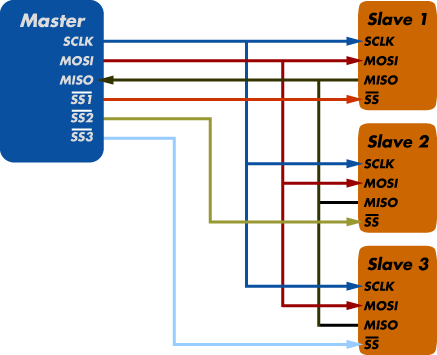
\includegraphics[scale=0.4]{spi.png}
\caption{Scheme of SPI communication}
\label{fig:spi}
\end{figure}


Usually the master is a microcontroller  or any processing unit that support SPI communication. To manage all 17 slave devices,  it is necessary a microcontroller with sufficient number of pins.   The microcontroller must be able not only to read the correct data from the IMUs but also it must send  data packages to the PC, in which the Magdwick Filter is implemented.   \\
\newline

\noindent $\bullet$ \textbf{PSoC 5LP} \textsuperscript \textregistered

\noindent The processing unit used was \textit{PSoC 5LP} developed by  Cypress Semiconductor. PSoC is a low power  ARM \textsuperscript \textregistered Cortex - M3 based programmable system on chip devices offering unmatched high-precision analog and the flexibility to design custom system solutions. When combined with the free PSoC software development tools (PSoC Creatortm and
PSoC Programmer) from Cypress, this module is more than sufficient for creating anything from basic microcontroller with embedded analog and digital functions to a highly complex system controller. Both the hardware system architecture and the software are supported by the PSoC
software tools. 
The PSoC integrated circuit is composed of a core, configurable analog and digital blocks, and programmable routing and interconnect. The configurable blocks in a PSoC are the biggest different from other microcontrollers, for this reason can be associated to the FPGA microcontroller family (Field-Programmable Gate Array). 
\begin{figure}[h]
\centering
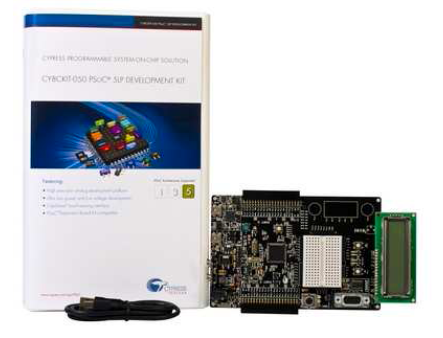
\includegraphics[scale=0.5]{psoc.png}
\caption{PSoC 5LP}
\label{fig:psoc}
\end{figure}

By using configurable analog and digital blocks, it is possible to  create and change mixed-signal embedded applications. These blocks are designed by PSoC-Creator, an Integreted Design Environment (IDE).  
The development of the PSoC 5LP  and PSoC-Creator has permitted to managed  the IMUs easily. 

The PSoC5 was exploited to read data from the slave devices allowing a SPI communication. The SPI bus could be only one, but were preferred three separated bus to have greater control on the hardware system. 

The informations from accelerometers, gyros and magnetometer were stored in the  memory of the PSoC5 ready to be sent to the PC.  The PSoC5 has a dual-channel USB interface to the host PC. Channel A of the highspeed USB interface is connected to the PSoC 5 in FIFO parallel mode to allow for the fastest possible transfers between the USB host and the PSoC 5. Channel B of the high-speed USB interface is connected to the PSoC 5 in serial mode to allow for UART communication between the host PC and the PSoC5. Using channel B USB, the PsoC can be read to the PC how a COM port, but to use this port presents an important disadvantage, the data-set can not sent if it is larger than 64 byte. For this reason another strategy was implemented. \\
\newline

\noindent $\bullet$ \textbf{Serial communication}

The communication between PSocC5 and PC was created exploiting the serial adapter 990 004. It is optimum to connect microcontroller and locig circuit to a PC. The heart of the integrated is the chip FT232R distributed by FTDI the supply a tension of 3.3V, thus it possible to connect the device to another TTL peripheral o microcontroller in the range of 3.3V-5V without the problem to convert the signal RS232 to  the TTL. The size of the circuit are very small, 25x18 mm and
\begin{figure}[h]
\centering
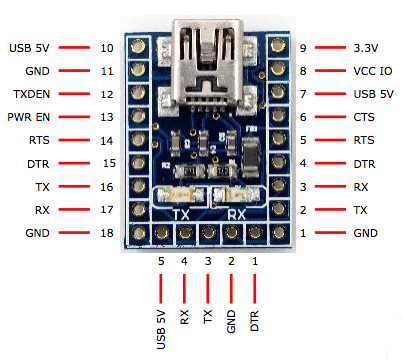
\includegraphics[scale=0.3]{usb_serial.png}
\caption{Serial adapter}
\label{fig:serial_adapter}
\end{figure}
two led visualize  input-output data of serial port, useful to continually supervise data stream escaping possible software/hardware problems. The device is USB 2.0 compatible and it permits all velocity to 1Mb. 

\begin{figure}[h]
\centering
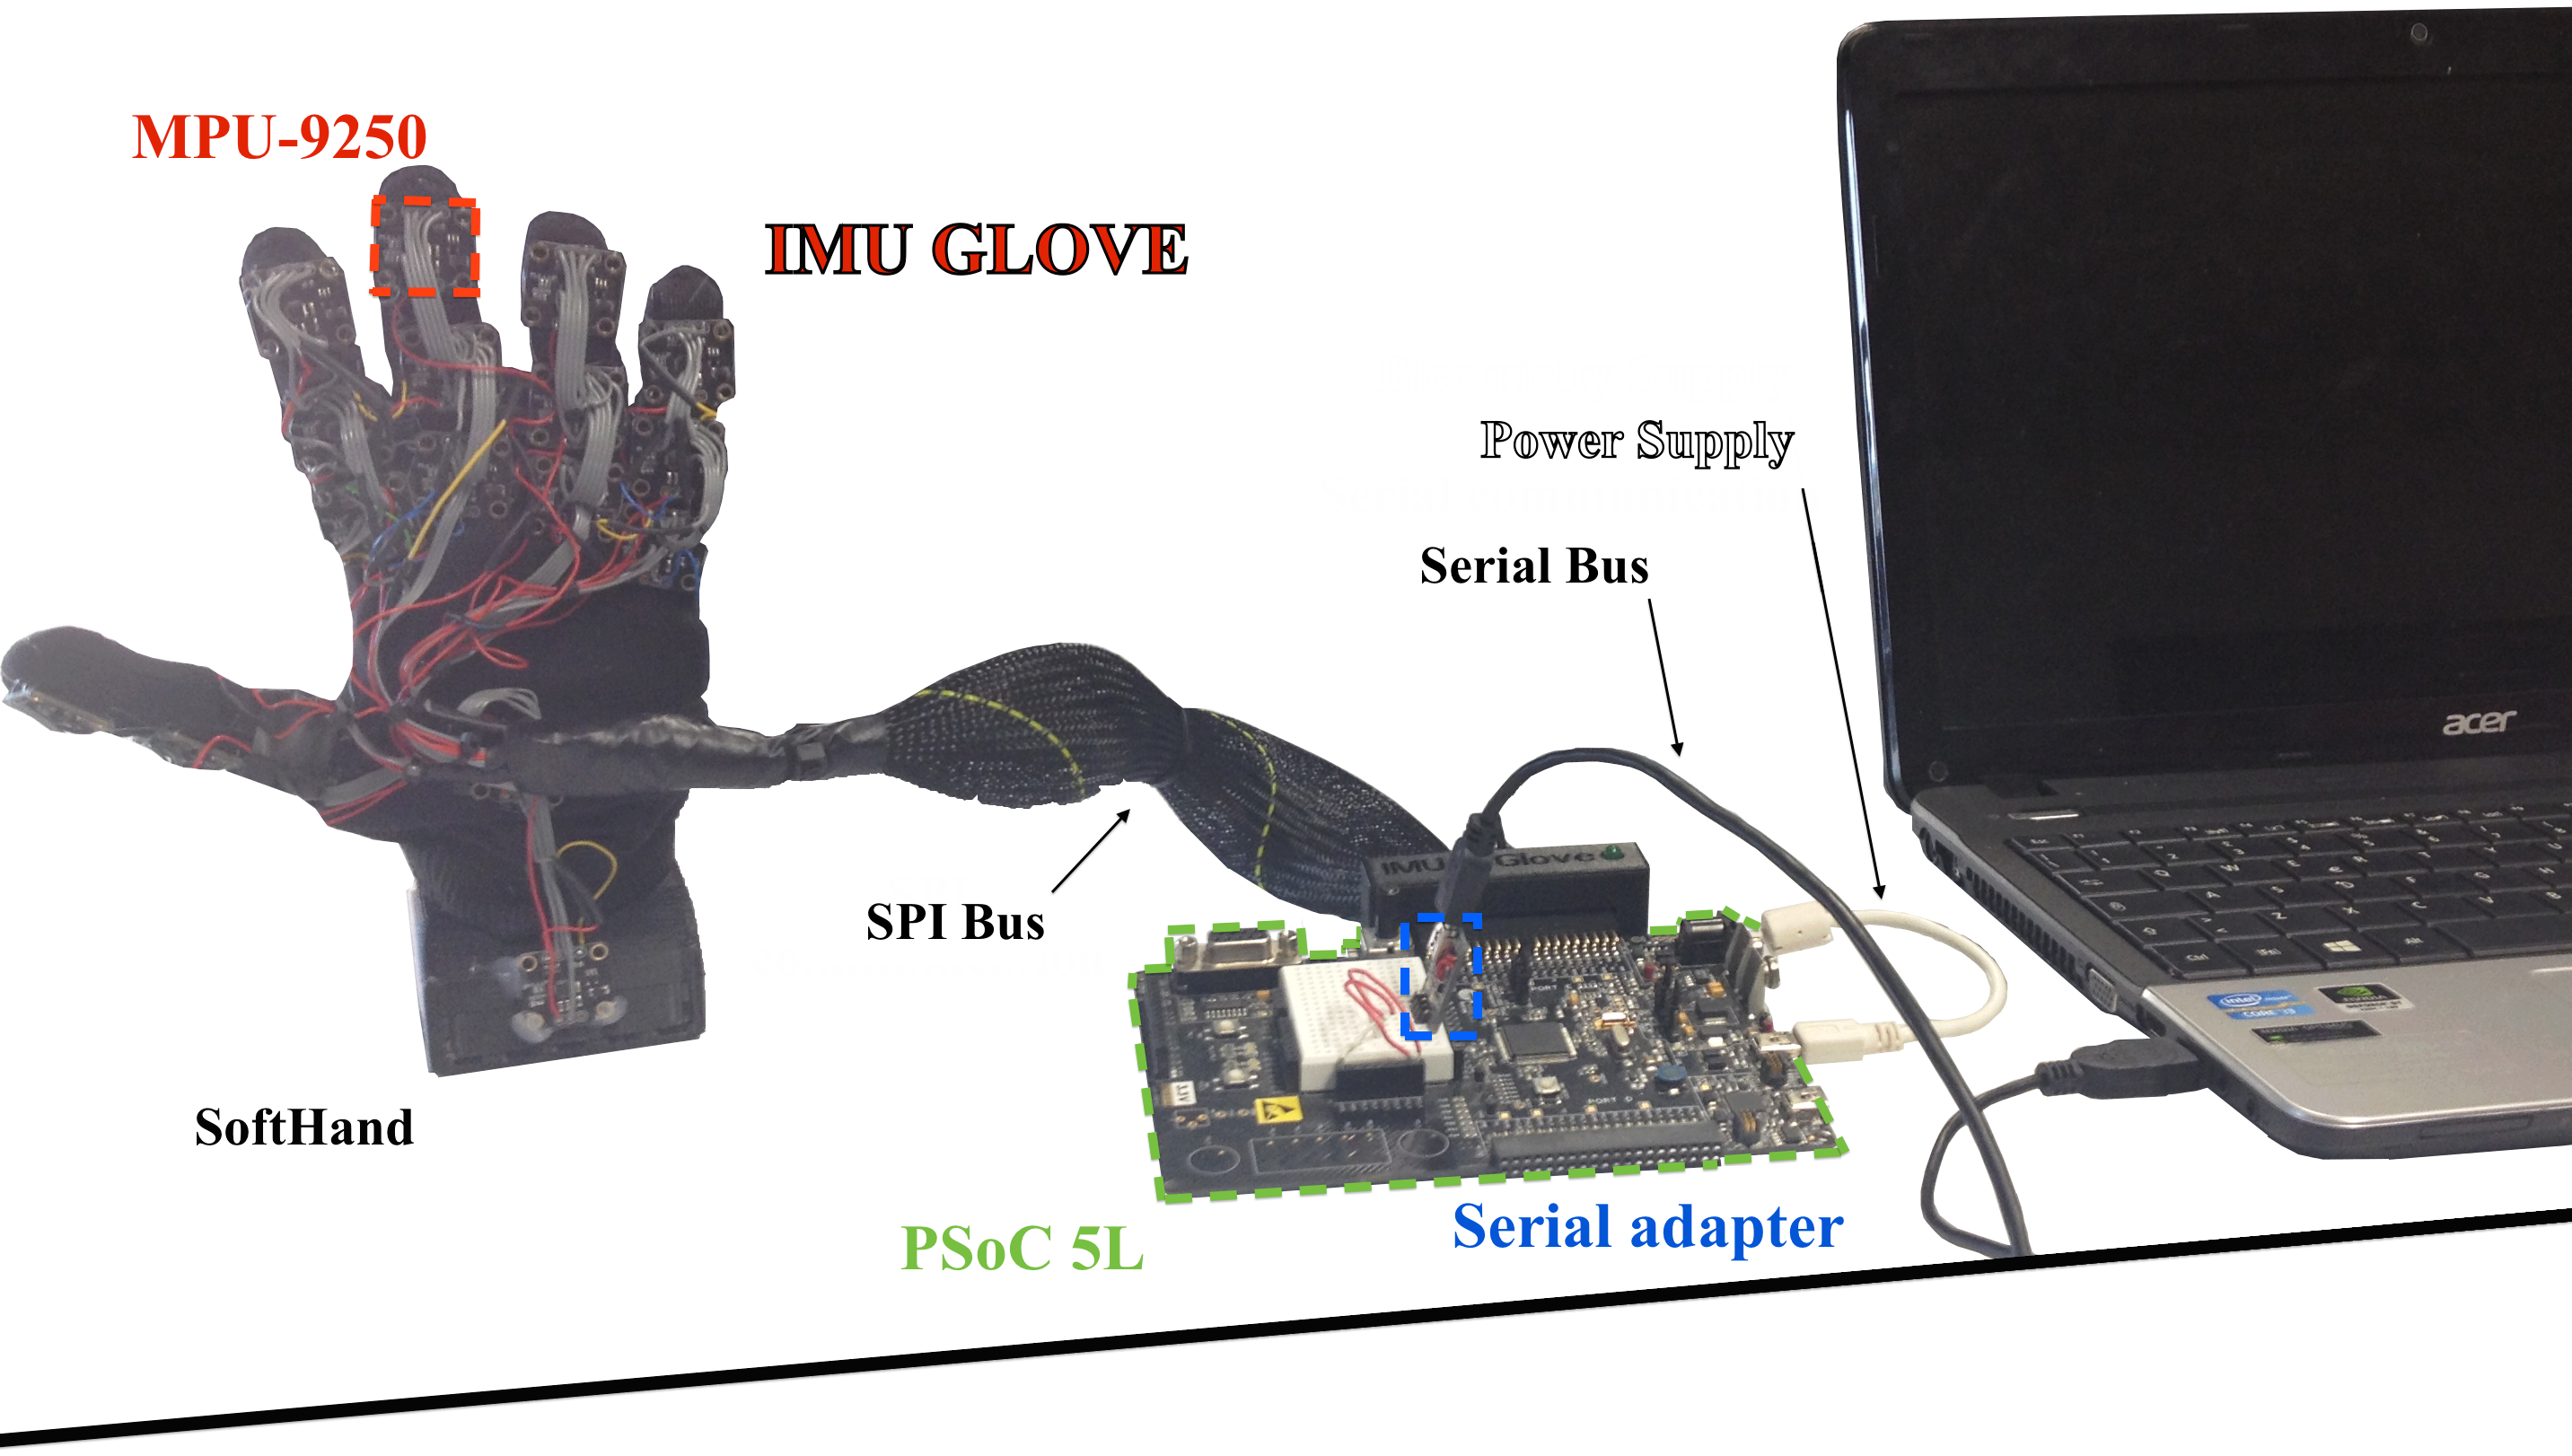
\includegraphics[scale=0.125]{hardware.png}
\caption{Full Hardware}
\label{fig:hardware}
\end{figure}


\noindent $\blacktriangleright$  \textbf{Code} \\ %\setlength{\headheight}{15pt}  \
\newline

The hardware described was managed in two fundamental step.  From one side there was the necessity to read IMU data and send its to computer, from the other side the sensor informations must be used to implement the algorithm for the  hand posture reconstruction.  
This was possible exploiting the PSoC5L where the \textit{Firmware} was installed and the \textit{Software} written in C++ in a Personal-Computer.

 \noindent $\bullet$ \textbf{Firmware}

 


\noindent $\bullet$ \textbf{Software}
